\chapter{Antecedentes} \label{Chapter:2}

\section{Inteligencia Emocional Artificial}

El término de inteligencia emocional, popularizado gracias a la publicación de Daniel Goleman en 1995 sobre cómo los efectos de esta característica afectiva pueden influir notablemente en las decisiones cotidianas y puesto al mismo nivel que el coeficiente intelectual, se define como la capacidad de identificar, evaluar y controlar ciertas características emocionales propias y ajenas, tales como el estado de ánimo, la motivación, la frustración, la angustia, los impulsos no racionales o la empatía \cite{Goleman}.

A pesar de ello, hasta la fecha, los investigadores que están intentando desarrollar ordenadores inteligentes se han centrado principalmente en la resolución de problemas, en el razonamiento, en el aprendizaje, en la percepción, en el lenguaje y en otras tantas tareas cognitivas de interés para este campo. De hecho, la mayoría de ellos no han tenido en cuenta la importante influencia de las emociones en estas funciones, y más cuando hay ciertas evidencias de que éstas juegan un papel fundamental en las atribuciones consideradas esenciales para la inteligencia en los humanos \cite{EmotionalIntelligence}. Por ello, este nuevo enfoque indica una clara necesidad de reconsideración del rol de las emociones en los ordenadores.

En este contexto, y en el intento de las computadoras de identificar el estado afectivo de un individuo, el sistema de reconocimiento ideal debería reunir las capacidades visuales y auditivas para capturar las expresiones faciales, los gestos y la entonación vocal con el fin de ser lo más riguroso posible. De forma adicional, otros aspectos que podrían enriquecer el resultado de la decisión final son la lectura de la temperatura corporal a través de la radiación infrarroja que emiten los cuerpos humanos, la medición de la actividad electrodérmica o la conductancia de la piel y el pulso \cite{Biosignals}.

Por lo tanto, es muy importante para la inteligencia afectiva artificial desarrollar formas de medir y aunar adecuadamente estas modulaciones, ya que pueden conducir a una mejor comprensión del estado emocional del sujeto. A pesar de ello, en este proyecto tan sólo se profundizará en el reconocimiento de las expresiones faciales, que individualmente se constituye como el módulo de mayor entropía desde el punto de vista de la identificación emocional.

\subsection{Reconocimiento de Expresiones Faciales}

\begin{figure}
    \centering
    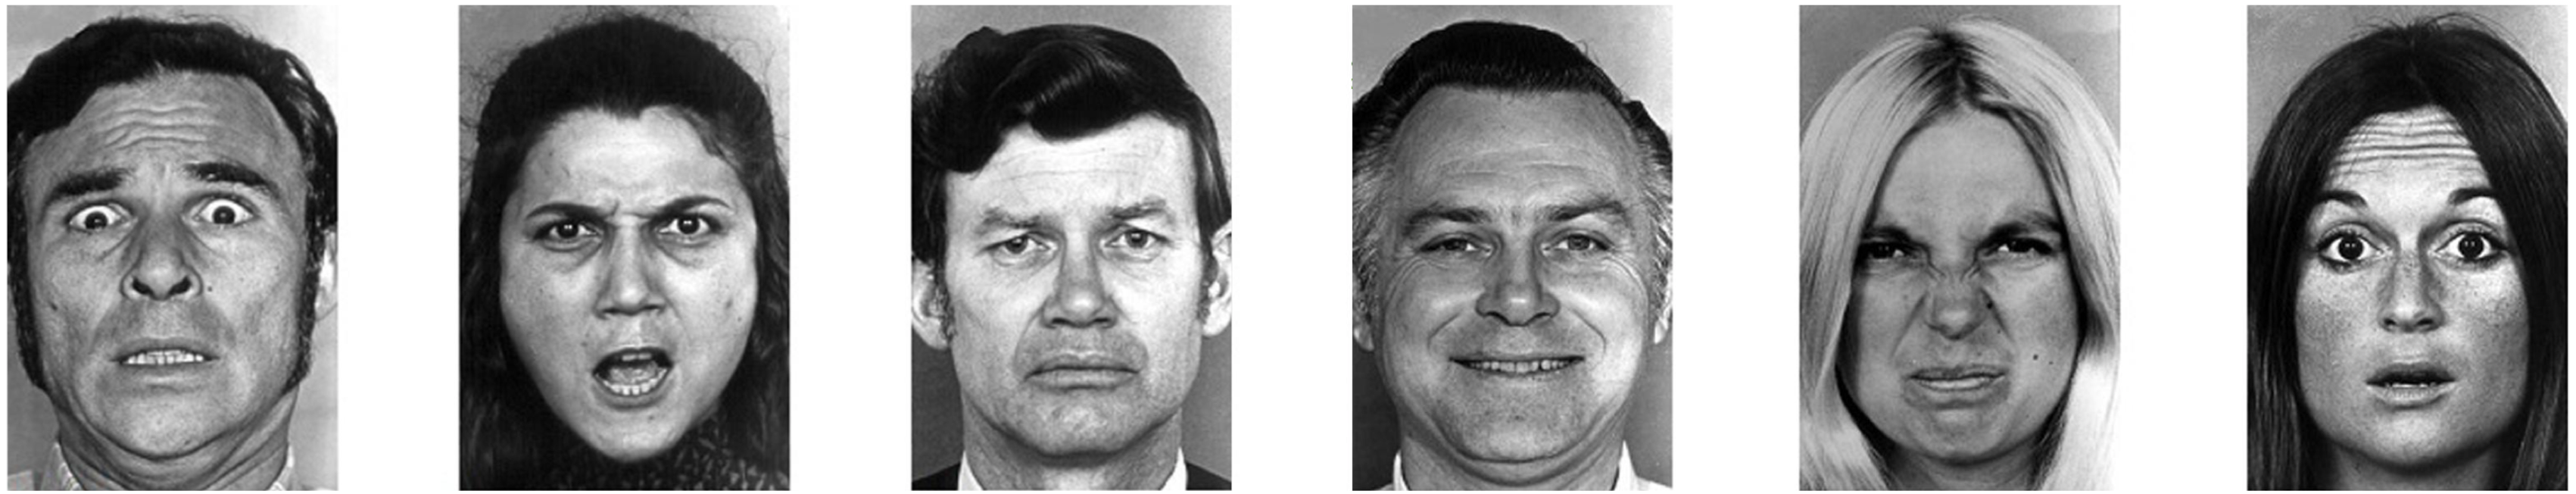
\includegraphics[width=\textwidth]{Images/emotions.png}
    \caption{Emociones universales propuestas por Paul Ekman (de izquierda a derecha: miedo, ira, tristeza, alegría, asco y sorpresa) \cite{Ekman}.}
    \label{fig:emotions}
\end{figure}

Paul Ekman, la principal autoridad de las expresiones faciales en el ámbito de la psicología, ha argumentado la existencia de seis emociones básicas  (ira, asco, miedo, alegría, tristeza y sorpresa) \cite{Ekman}, mostradas en la \autoref{fig:emotions}. Cada una de ellas tiene un conjunto de patrones únicos en el movimiento muscular facial. Estos patrones, así como su estudio detallado e identificación, posteriormente han sido integrados en un sistema de codificación facial (FACS) \cite{FACS}, el cual proporciona las técnicas necesarias para asociar los músculos del rostro a su espacio emocional correspondiente. De hecho, gran parte de los intentos de automatizar el reconocimiento de las expresiones faciales, capaces de ofrecer una identificación automática y en tiempo real a partir de un análisis tridimensional de la cara del sujeto, se basan en este sistema \cite{FaceReader}.

Por otro lado, en los últimos años, y gracias principalmente a la irrupción y al enorme progreso que ha experimentado el campo del aprendizaje profundo y automático en el ámbito del reconocimiento visual \cite{DeepLearning}, se han comenzado a desarrollar nuevas técnicas y métodos de identificación de las expresiones faciales. Este hecho, además, ha supuesto un nuevo punto de inflexión en este entorno dados los espectaculares resultados obtenidos gracias a la implementación de estos nuevos modelos, cuya eficacia y rendimiento se van a intentar analizar y reproducir en este proyecto.

Por último, cabe destacar que actualmente ninguno de los modelos anteriormente descritos pretende reconocer las emociones subyacentes (una sonrisa forzada, por ejemplo), centrándose la identificación tan solo en la expresión del rostro del sujeto en un instante determinado.

\section{Aprendizaje Automático}

El aprendizaje automático es una rama de la inteligencia artificial y puede definirse como un área de estudio que proporciona a las computadoras la capacidad de aprender, sin éstas estar explícitamente programadas \cite{MachineLearning}. De esta forma, mediante los variados algoritmos de aprendizaje automático es posible generar un resultado, generalmente un conjunto de predicciones o decisiones, a partir de diversos datos de entrada sin la necesidad de agregar nuevas líneas de código al sistema inicial.

En lo que respecta al proceso de aprendizaje del modelo en sí, es posible distinguir tres categorías por las que se rige este procedimiento y cuya clasificación está basada en el tipo o en la existencia de retroalimentación durante el entrenamiento:
\begin{itemize}
  \item \textbf{Aprendizaje supervisado}. Se caracteriza por la recepción de un conjunto de entradas etiquetadas, las cuales son atribuidas a la clase de pertenencia correspondiente gracias al algoritmo de aprendizaje pertinente. En este proceso de asignación el modelo va adaptándose o modificando sus parámetros con el fin de ofrecer un mejor rendimiento.
  \item \textbf{Aprendizaje no supervisado}. En este caso se recibe un conjunto de entradas sin etiquetar, por lo que el modelo intenta aprender de estos datos de entrada mediante la exploración de los patrones existentes en ellos.
  \item \textbf{Aprendizaje por refuerzo}. Se distingue por implementar un sistema de recompensa o castigo en función de las decisiones que un agente de \textit{software} ha tomado en un entorno dado para alcanzar un objetivo concreto.
\end{itemize}

Particularmente en este proyecto y tal y como se podrá comprobar durante los siguientes capítulos, el planteamiento del problema del reconocimiento de emociones desde el punto de vista de las herramientas y de los conjuntos de datos empleados en este trabajo implica un acercamiento hacia la utilización de técnicas de aprendizaje supervisado.

\subsection{Redes Neuronales Artificiales} \label{Chapter:ANN}

El aprendizaje supervisado tiene un conjunto de herramientas enfocadas a resolver problemas dentro de su dominio, siendo una de ellas, precisamente, las Redes Neuronales Artificiales (ANN).

\begin{figure}
    \centering
    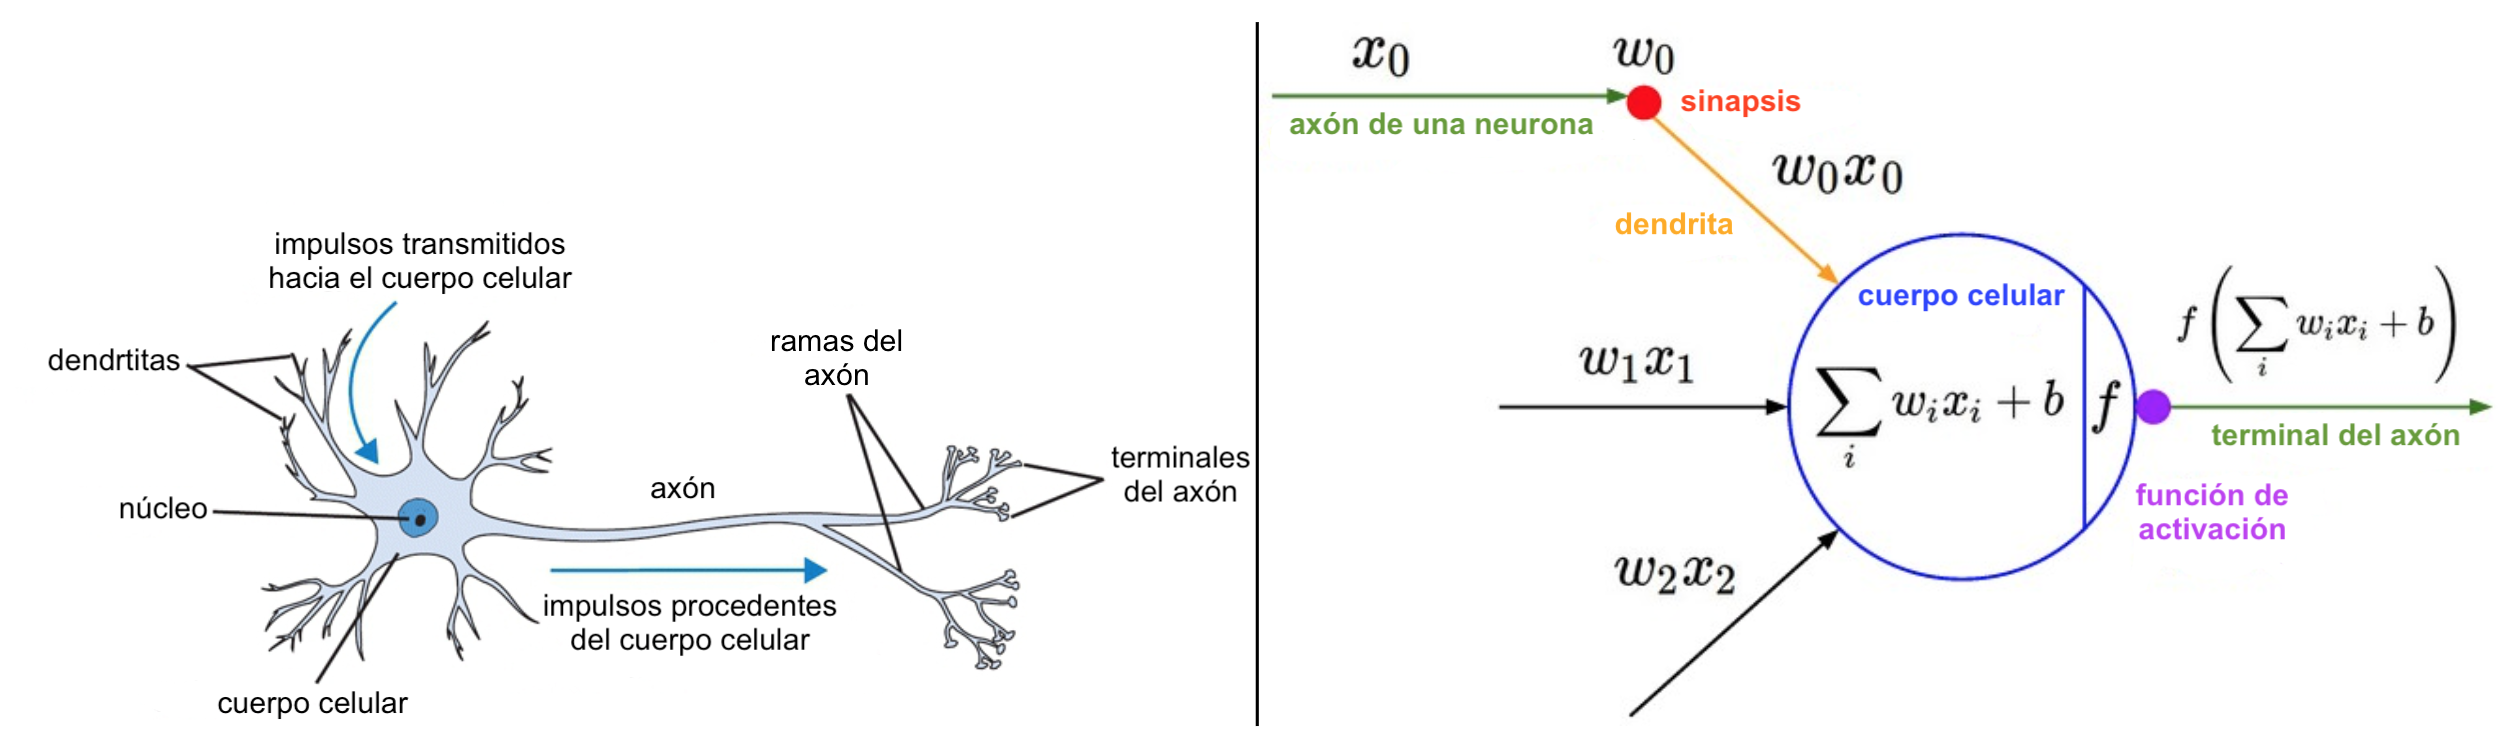
\includegraphics[width=\textwidth]{Images/analogy-neuron.png}
    \caption{Imagen de una neurona biológica (izquierda) y el modelo matemático que intenta reproducir superficialmente su funcionamiento (derecha) \cite{CS231n}.}
    \label{fig:analogy}
\end{figure}

Estas redes son un modelo computacional vagamente inspirado en las redes neuronales biológicas que constituyen los cerebros humanos \cite{ANN} y cuya analogía con el modelo matemático se puede observar en la \autoref{fig:analogy}. Cada una de estas neuronas recibe una serie de señales de entrada en sus dendritas y produce determinadas señales de salida que son trasladadas a lo largo del axón, el cual posteriormente se bifurca y se conecta a través de la sinapsis a las dendritas de otras neuronas. En el modelo computacional, por su parte, las señales que se desplazan a lo largo de los axones ($x_i$) interactúan de forma multiplicativa ($\omega_i\cdot x_i$) con las dendritas de otras neuronas en función de las fuerzas sinápticas (los pesos $\omega_i$), que son precisamente los elementos aprehensibles de los algoritmos de aprendizaje automático. Estos pesos, por lo tanto, son los que controlan la intensidad y la dirección (sinapsis excitatoria --peso positivo-- o inhibitoria --peso negativo--) de influencia de una neurona sobre otra. En el modelo biológico, las dendritas trasladan estas señales provenientes de otras neuronas al cuerpo celular, donde su suma da lugar a un potencial excitatorio postsináptico, que en caso de superar un determinado umbral causará la generación de un impulso eléctrico o potencial de acción que será enviado a largo del axón de la propia neurona. Este proceso en el modelo computacional es menos complejo al considerar que la información se encuentra tan sólo en la frecuencia de disparo del potencial de acción. En base a esta interpretación, la descarga de una neurona artificial se modela con una función de activación no lineal que representa la frecuencia de los impulsos a lo largo del axón, es decir, se toma como entrada la intensidad de la señal después de la suma ($\sum\limits_{i=0}^n \omega_i\cdot x_i + b$) y se normaliza, típicamente, según el tipo de función de activación, obteniéndose una salida acotada. Cabe destacar que el parámetro $b$, ignorado en los próximos capítulos por razones de simplificación, es necesario para evitar interrupciones en el proceso de aprendizaje cuando las entradas inyectadas ($x_i$) son nulas.

\begin{figure}
    \centering
    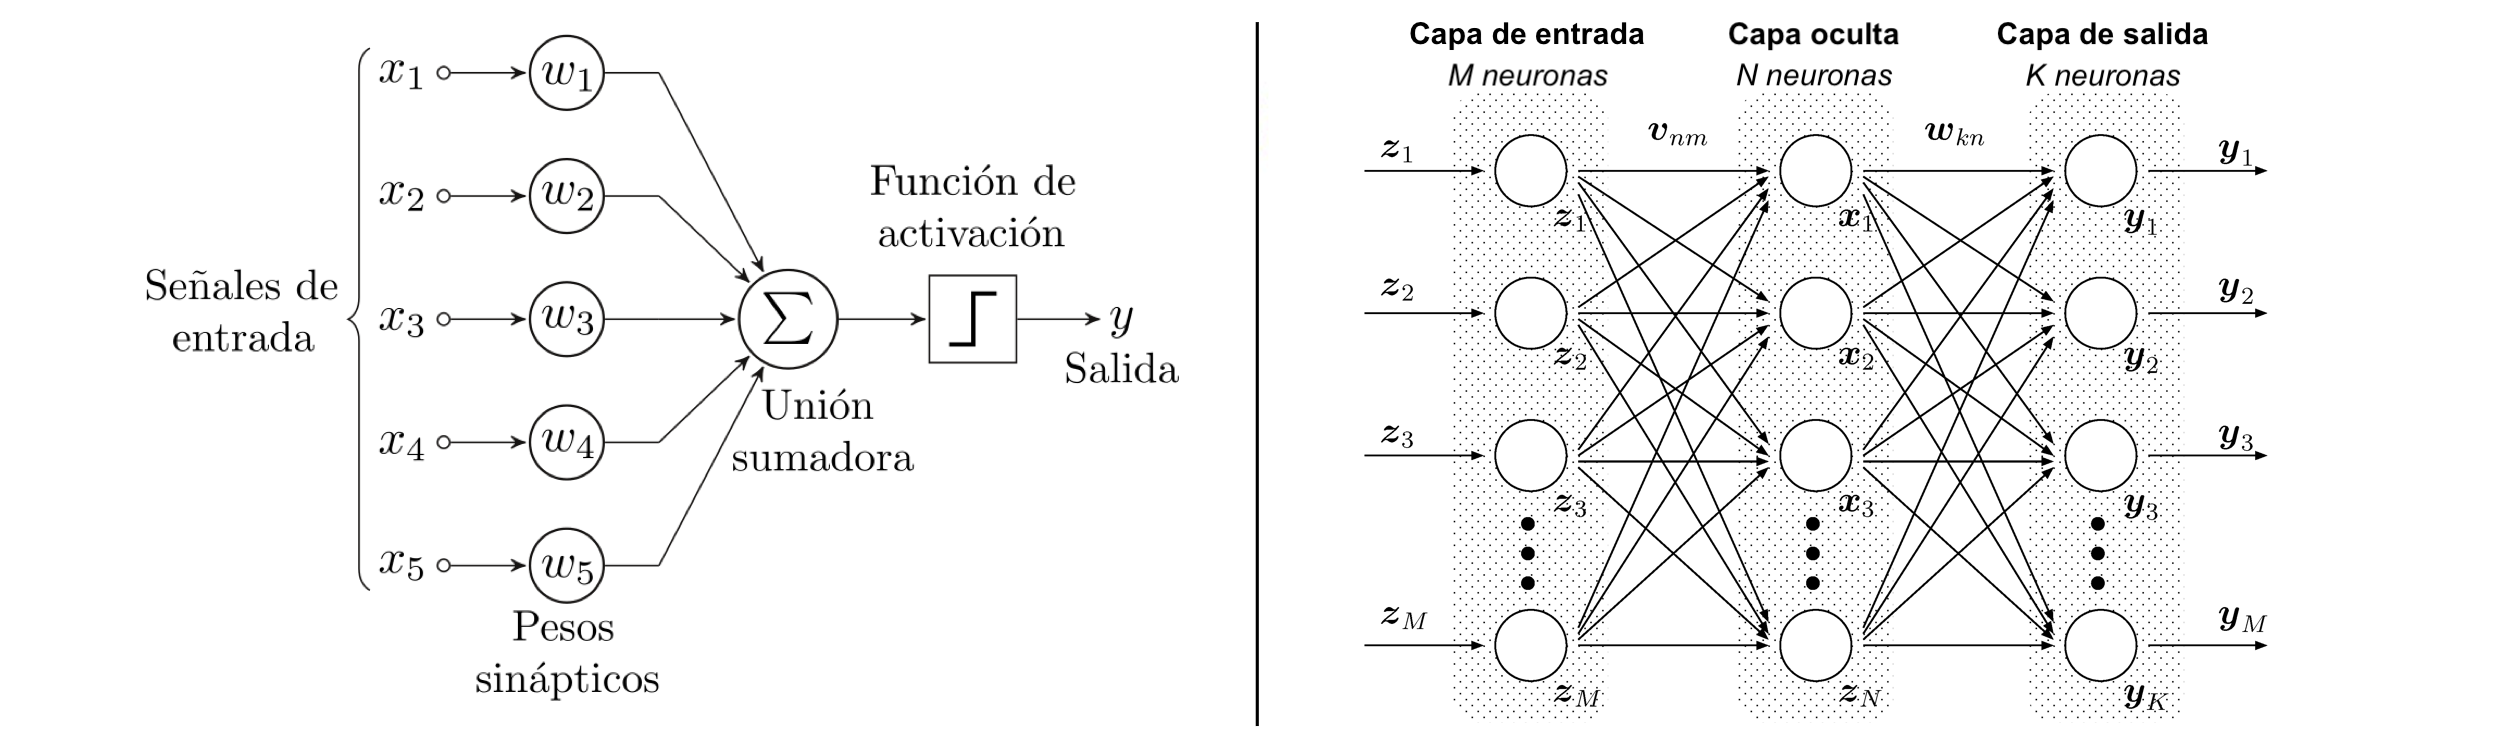
\includegraphics[width=\textwidth]{Images/perceptron_MLP.png}
    \caption{Topología de un perceptrón simple (izquierda) \cite{img:perceptron} y de un MLP con una capa oculta (derecha) \cite{img:MLP}.}
    \label{fig:ANN}
\end{figure}

Una ANN, por lo tanto, es una red estratificada de estas neuronas artificiales, pudiendo consistir en una capa de entrada, capas ocultas y una capa de salida \cite{Engelbrecht}. Las estructuras más básica de una ANN, el perceptrón y el perceptrón multicapa (MLP), que permite resolver problemas que no son linealmente separables, se representan en la \autoref{fig:ANN}.

En definitiva, una ANN es un conjunto de funciones que realizan una predicción que es expresada, generalmente, como una distribución de probabilidad para todas las etiquetas. Esta predicción, posteriormente, es cuantificada con respecto al valor real correspondiente, obteniéndose una función de error o de pérdidas, la cual es utilizada para actualizar los pesos de las distintas capas con el fin de mejorar la predicción global. Esto se lleva a cabo, tradicionalmente, mediante el método de propagación hacia atrás de errores o retropropagación y cuyas características se analizarán en profundidad en la \autoref{Chapter:Backpropagation}.

En cuanto al contexto histórico, las unidades neuronales fueron reconocidas por primera vez como elementos funcionales del sistema nervioso a finales del siglo XIX a través del trabajo de Santiago Ramón y Cajal. Mediante su estudio, gracias al cual obtuvo el Premio Nobel, propuso que estas células discretas interconectadas establecían una red compleja para la transmisión de la información. Esta descripción se conoce como la doctrina de la neurona y es el modelo aceptado a día de hoy en neurofisiología.

Posteriormente, estas redes, pese a formularse como un modelo para la realización de cálculos matemáticos en la década de los cuarenta \cite{McCulloch}, no fueron implementadas como tales hasta finales de los cincuenta, cuando fue presentada la arquitectura más simple de las ANN: el perceptrón \cite{Rosenblatt}. Este estaba formado por una serie de capas que contaban con un número determinado de nodos, cada uno de los cuales, excepto los de la entrada, representaban justamente a una neurona biológica. Además, fue en este artículo  en el que se introdujo precisamente la técnica de aprendizaje supervisado denominada retropropagación para entrenar las redes neuronales artificiales. 

A pesar de este gran paso, las limitaciones computacionales y de \textit{hardware} de la época (también existentes hoy en día), así como un enfoque de la investigación en inteligencia artificial hacia las representaciones simbólicas de los problemas, hizo que no fuera hasta principios de la década de los noventa cuando estas redes neuronales artificiales volvieran a cobrar protagonismo. Los responsables de ello fueron diversas publicaciones de una serie de modelos que explotaban las ANN, como la NETtalk \cite{NETtalk}, que mediante el aprendizaje automático fue capaz de aprender a leer en voz alta, o la ANN de múltiples capas desarrollada por Yann LeCun \cite{MNIST}, que permitía el reconocimiento de dígitos escritos a mano tomados de los códigos postales. Esta última publicación, de hecho, fue la pionera en integrar el reconocimiento de imágenes y el aprendizaje automático en un mismo modelo, además de introducir una serie de conceptos que posteriormente serían clave en el desarrollo de las Redes Neuronales Convolucionales (CNN), tales como la asignación de objetos según sus características a una serie de clases o la compartición de los pesos.

Cabe destacar que durante esta década muchos investigadores preferían utilizar las Máquinas de Vectores de Soporte (SVM) en las tareas de aprendizaje supervisado, cuya simplicidad y resultados eclipsaban a las ANN. Sin embargo, esta situación cambiaría drásticamente a partir del año 2010, cuando el desarrollo de potentes y asequibles herramientas de \textit{software} y de \textit{hardware}, junto con la existencia de una enorme cantidad de datos a explotar, posibilitaron la realización de cálculos extremadamente grandes sobre modelos complejos, obteniéndose unos resultados sin precedentes y que marcarían el auge del aprendizaje profundo.

\section{Aprendizaje Profundo}

El último resurgimiento de las ANN se conoce como aprendizaje profundo, término cuya definición puede englobarse en los siguientes puntos estrechamente relacionados \cite{def:DeepLearning}:
\begin{itemize}
  \item Es una clase de técnicas de aprendizaje automático que permite la explotación de un gran número de capas que procesan la información de forma no lineal para la extracción, transformación, análisis  y clasificación de patrones.
  \item Es un subcampo dentro del aprendizaje automático basado en algoritmos cuya función es aprender los múltiples niveles de representación de la información de la entrada con el fin de poder modelar relaciones complejas entre los datos en una arquitectura profunda, definiéndose los conceptos del nivel superior a partir de los del nivel inferior.
  \item Es una nueva área de investigación del aprendizaje automático introducida con el objetivo de acercar este subcampo de las ciencias de la computación a uno de sus objetivos originales: la inteligencia artificial. 
\end{itemize}

Estas técnicas y métodos que permiten aprender determinadas características por sí mismos a partir de representaciones sencillas han tenido un especial éxito en campos como la visión por computador, el procesamiento del lenguaje natural y el reconocimiento automático de voz. En el área del reconocimiento visual artificial, por ejemplo, una ANN puede alimentarse con los píxeles de una imagen, determinando posteriormente el algoritmo de aprendizaje si esta específica combinación representa cualquier característica particular que es repetida a través de una o varias imágenes.

Por otro lado, el hecho de que hoy en día ya no se emplee el término de ANN, sino el de aprendizaje profundo, se debe principalmente al impulso que recibió el campo de la inteligencia artificial gracias al trabajo de Geoffrey Hinton. Fue precisamente su publicación de 2012 sobre el reconocimiento automático de voz \cite{Hinton}, con la colaboración de los grupos de investigación de la Universidad de Toronto, Micrososft Research, Google Research e IBM Research, la primera que contenía una implementación directa en el ámbito industrial de las técnicas de aprendizaje profundo.

En lo que respecta al ámbito de la visión por computador, el punto crítico también llegaría de la mano de Hinton dentro del contexto del Desafío del Reconocimiento Visual a Gran Escala (ILSVRC) \cite{ILSVRC}. Esta competición consiste en evaluar el desempeño de los modelos de los participantes en la clasificación de 100\,000 fotografías etiquetadas a mano con la presencia o ausencia de 1\,000 categorías de objetos diferentes. Su creación en 2010, así como de la base de datos ImageNet utilizada para el entrenamiento, tenían como objetivo motivar la investigación de \textit{software} enfocado al campo del reconocimiento visual. De hecho, el avance experimentado tan sólo dos años después de la aparición del ILSVRC es considerado ampliamente como el comienzo de la revolución del aprendizaje profundo, tanto en el entorno de investigación de la inteligencia artificial como en el de la industria tecnológica \cite{AIboom}. Este progreso estuvo marcado por la presentación, por parte de Alex Krizhevsky, Ilya Sutskever y Geoffrey Hinton, de un modelo capaz de reducir a la mitad la tasa de error existente en ese momento \cite{Krizhevsky}. El sistema desarrollado combinaba varios elementos críticos que se convertirían en los pilares fundamentales de los modelos de aprendizaje profundo: el entrenamiento mediante las Unidades de Procesamiento Gráfico (GPUs), las Redes Neuronales Convolucionales (CNN), el empleo de la Unidad Lineal Rectificada (ReLU) y del método para evitar el sobreentrenamiento, conocido como \textit{dropout}.

\subsection{Empleo de las Unidades de Procesamiento Gráfico}

Probablemente el componente más relevante e influyente dentro del explosivo progreso del aprendizaje profundo haya sido el uso de las Unidades de Procesamiento Gráfico en el entrenamiento de los modelos diseñados.

\begin{figure}
    \centering
    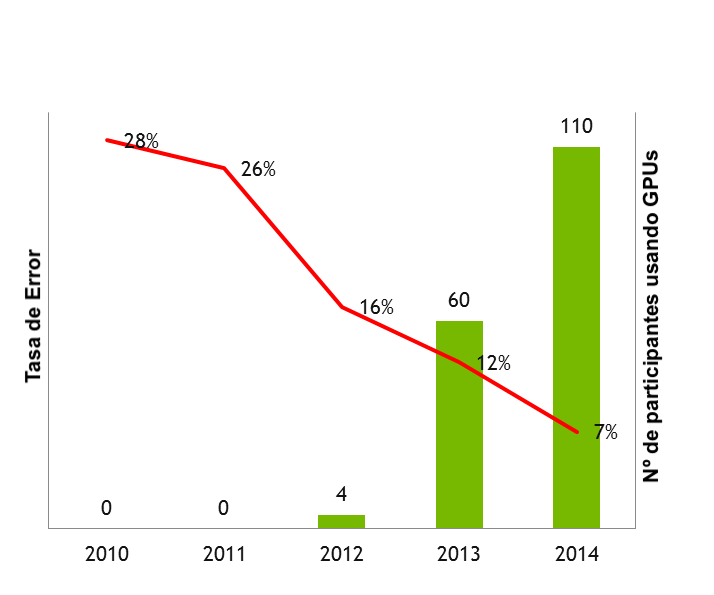
\includegraphics[scale=0.8]{Images/ILSVRC.png}
    \caption{Tasa de error de la entrada ganadora del ILSVRC (línea roja) y número creciente de entradas que usan GPUs cada año (barras verdes).\cite{img:ILSVRC}}
    \label{fig:ILSVRC}
\end{figure}

Las GPUs son esencialmente calculadoras de coma flotante cuya arquitectura paralela de miles de núcleos ofrece la posibilidad de manejar múltiples tareas simultáneamente. Esta capacidad de paralelización, precisamente, es la que ha sido ampliamente explotada por los algoritmos de aprendizaje profundo en la realización de operaciones vectoriales y matriciales, logrando una reducción de los tiempos de entrenamiento en unas 10 -- 20 veces \cite{DeepLearning}. Esto ha posibilitado, a su vez, el entrenamiento de modelos significativamente más complejos o profundos y por lo tanto, la obtención de tasas de error cada vez más bajas.

El desarrollo experimentado y su influencia pueden apreciarse en la \autoref{fig:ILSVRC}, que muestra como los resultados del ILSVRC van mejorando a medida que se populariza el uso de las GPUs. Destaca también la caída precipitada del año 2012 propiciada por la implementación de la red AlexNet, modelo que se ha descrito brevemente en el apartado anterior y que ha revolucionado el reconocimiento e identificación visual, siendo especialmente relevante en este proyecto.

\section{Redes Neuronales Convolucionales} \label{Chapter:CNN}

Las investigaciones sobre la corteza visual animal, cuyos primeros estudios trascendentales datan de 1968 con la publicación de Hubel y Wiesel sobre los campos receptivos y la arquitectura funcional del córtex visual de los monos \cite{Hubel}, están estrechamente relacionadas con el desarrollo de las redes neuronales convolucionales. Fue precisamente en este estudio en el que se describió por primera vez cómo las señales obtenidas por los ojos son procesadas por parcelas visuales en el neocórtex para generar detectores de bordes, de movimientos, de profundidad y de color, construyendo bloques de la escena visual.

Una de las primeras implementaciones inspiradas en este estudio fue el Neocognitron \cite{Neocognitron}. Este modelo de red neuronal intentaba imitar el funcionamiento de los dos tipos de células introducidas en el anterior documento: las células simples, que responden principalmente a bordes y a líneas de orientaciones particulares y las células complejas, que presentaban campos receptivos más grande e invariancia local. A pesar de todo ello, este modelo presentaba un importante inconveniente en el proceso de aprendizaje al no haberse desarrollado, por aquella época, un método para ajustar los valores de los pesos con respecto a una medida de error para toda la red, como la retropropagación. Esta técnica de propagación hacia atrás de errores, analizada en \autoref{Chapter:Backpropagation}, no fue implementada en el entrenamiento de las ANN hasta 1985, cuando se publicó el trabajo de Rumelhart, Hinton y Williams \cite{Rumelhart}.

A partir de este momento se llevaron a cabo numerosas implementaciones con aplicaciones prácticas empleando la propagación hacia atrás de errores para entrenar las CNN, siendo Yann LeCun con su clasificador de dígitos escritos a mano (MNIST) \cite{MNIST} el pionero e inspirando, además, gran parte de las investigaciones futuras.

En cuanto a las redes neuronales convolucionales en sí, éstas son muy similares a las redes neuronales ordinarias tratadas en la \autoref{Chapter:ANN}: están formadas por neuronas que tienen pesos que se pueden aprender, reciben entradas a las que se aplica un producto escalar y opcionalmente una función no lineal, y obtienen, en la última capa, la puntuación de pertenencia a una determinada clase. La principal diferencia, por lo tanto, es que las arquitecturas convolucionales suponen explícitamente que las entradas son imágenes, haciendo que las operaciones sean más eficientes y reduciendo inmensamente la cantidad de parámetros en la red \cite{CS231n}. Además, las capas de una CNN tienen neuronas dispuestas en las 3 dimensiones: anchura, altura y profundidad, volumen que coincide, precisamente, con las dimensiones en píxeles (ancho y alto) y el modelo de color (profundidad), tradicionalmente RGB, de una imagen. Asimismo, las neuronas de una determinada capa de una CNN sólo están conectadas a una pequeña región de la capa anterior, en lugar de a todas las neuronas de una manera absolutamente conectada, como ocurría en las ANN. Es por ello que al final de la arquitectura de una CNN la imagen completa de la entrada se reduce a tan solo un vector de puntuaciones de pertenencia a una determinada clase dispuesto a lo largo largo de la dimensión de profundidad, tal y como se puede observar en la \autoref{fig:CNN}.

\begin{figure}
    \centering
    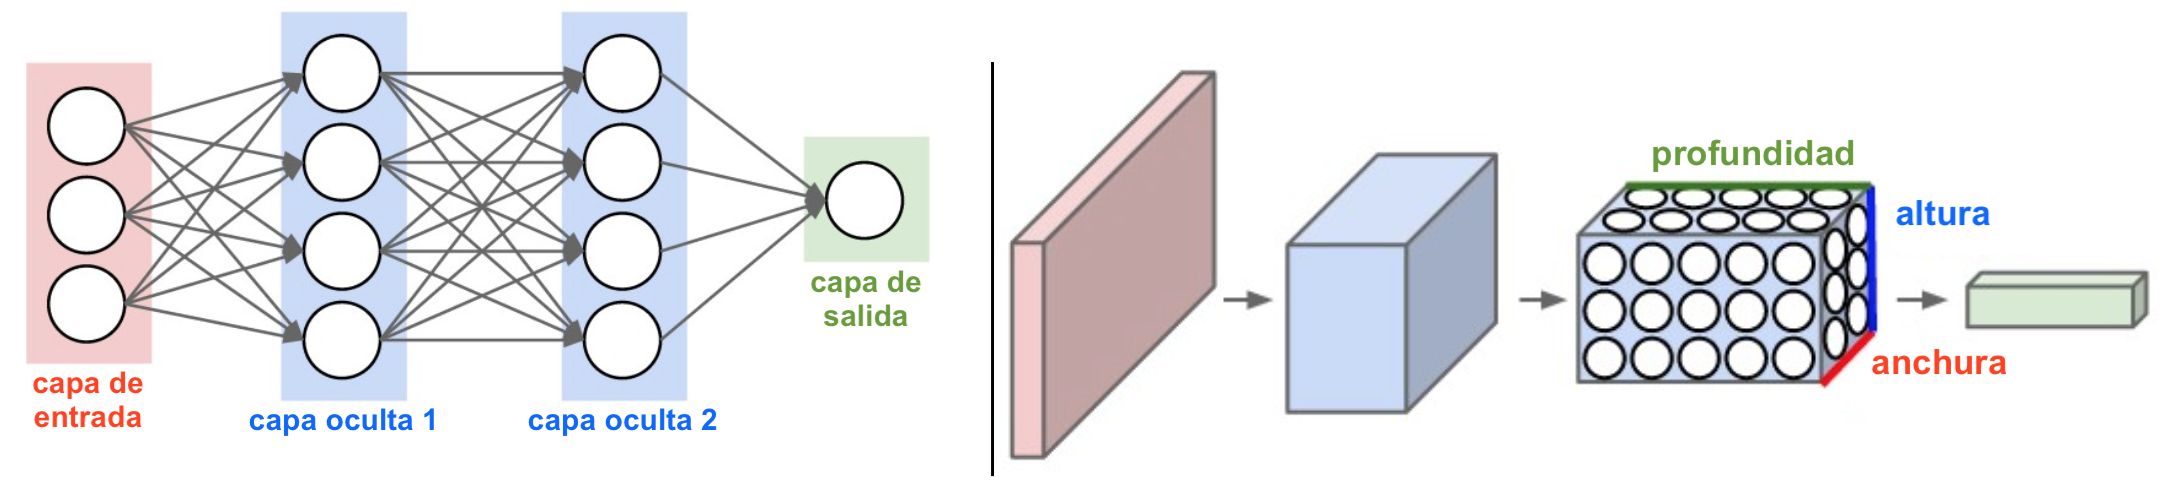
\includegraphics[width=\textwidth]{Images/CNN.png}
    \caption{Una ANN ordinaria de 3 capas (izquierda) y una CNN (derecha) \cite{CS231n}.}
    \label{fig:CNN}
\end{figure}

En definitiva, una CNN simple es una secuencia de capas que se encargan de transformar un volumen de activación en otro diferente a través de una función diferenciable. Generalmente, y particularmente en este proyecto, son utilizadas principalmente las capas descritas en \autoref{Chapter:Layers} (capas convolucionales, de agrupación o \textit{pooling}, íntegramente conectadas, etc.), con cuyo apilamiento sucesivo se va a pretender formar una arquitectura neuronal convolucional completa.

Algunas de estas arquitecturas, especialmente las más relevantes en el contexto de este proyecto, se enumeran a continuación:
\begin{itemize}
  \item \textbf{LeNet} \cite{LeNet-5}. Las primeras aplicaciones exitosas de las CNN fueron desarrolladas por Yann LeCun en la década de 1990. Entre ellas, la más conocida es la arquitectura LeNet, que se utilizó para leer los dígitos de los códigos postales.
  \item \textbf{AlexNet} \cite{Krizhevsky}. La publicación con la que se popularizó el uso de las CNN en el campo de la visión por computador fue la ya nombrada anteriormente AlexNet. Este modelo se presentó al desafío ILSVRC de ImageNet en 2012, superando al segundo finalista con una diferencia de más del 10\% en la tasa de error. En cuanto a su arquitectura, era muy similar a LeNet, con la diferencia de que presentaba capas convolucionales más profundas, más grandes y apiladas unas sobre otras, cuando lo común era tener capas convolucionales seguidas inmediatamente de capas de agrupación.
  \item \textbf{GoogLeNet} \cite{GoogleNet}. El ganador del ILSVRC 2014 fue una CNN desarrollada por el grupo de investigación de inteligencia artificial de Google. Su principal contribución fue la introducción de un modelo con el que se consiguió reducir drásticamente la cantidad de parámetros en la red, pasando a contar con tan sólo 4 millones, un número más que razonable teniendo en cuenta los 60 millones de la red AlexNet. También cabe destacar las posteriores versiones de GoogLeNet desarrolladas, como Inception-v3 e Inception-v4, que, como se verá en el \autoref{Chapter:5}, son fundamentales en el presente proyecto.
  \item \textbf{VGGNet} \cite{VGGNet}. Obtuvo el segundo puesto en el desafío ILSVRC 2014, aportando y desarrollando la idea de que la profundidad de la red es un componente crítico para la obtención de buenos resultados. Sin embargo, a pesar de  haber alcanzado una tasa de error más que razonable, este modelo presentaba una importante desventaja al contar con casi 140 millones de parámetros, haciéndolo muy costoso de entrenar y requiriendo, además, mucha memoria.
  \item \textbf{ResNet} \cite{ResNet}. Esta red residual fue la vencedora del ILSVRC 2015 al implementar una serie de conceptos clave como las conexiones directas entre capas no contiguas y la normalización por lotes, lo que además de acelerar la evaluación del modelo, favorecía la prevención del sobreaprendizaje. Actualmente, de hecho, las ResNet o sus variaciones son la opción predeterminada para implementar las CNN en la práctica \cite{ImpactResNet}.
\end{itemize}

\subsection{Retropropagación} \label{Chapter:Backpropagation}

\begin{figure}
    \centering
    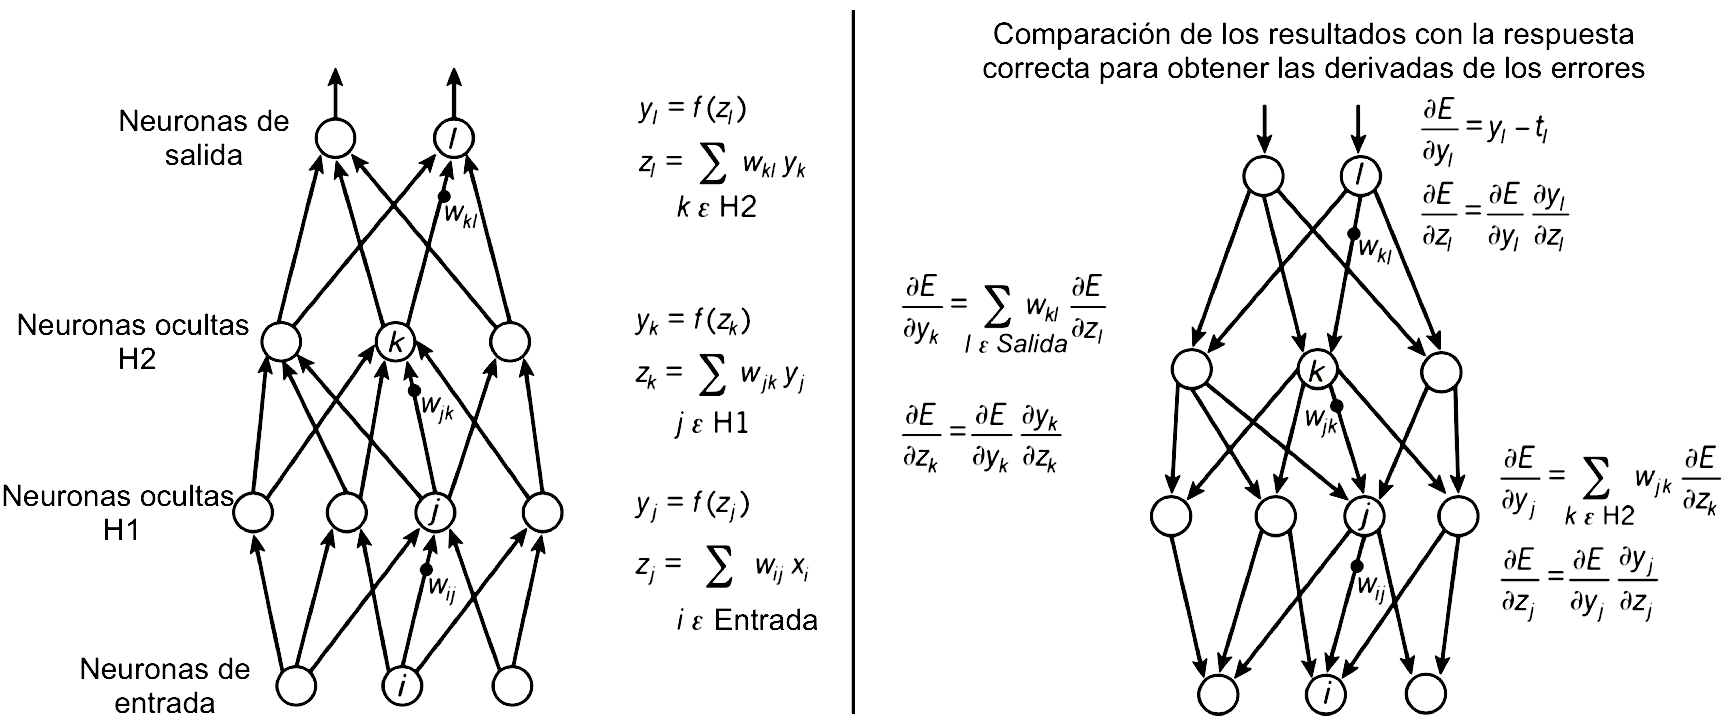
\includegraphics[width=\textwidth]{Images/backpropagation.png}
    \caption{Ecuaciones utilizadas para calcular las salidas o predicciones de una red neuronal con dos capas ocultas y una capa de salida (izquierda) y las ecuaciones empleadas en la retropropagación si la función de pérdidas para cada una de las unidades neuronales es $\frac{1}{2}\cdot (y_l - t_l)^2$, donde $t_l$ es el valor objetivo (derecha) \cite{DeepLearning}.}
    \label{fig:backpropagation}
\end{figure}

El procedimiento de la retropropagación para calcular el gradiente de una función de pérdidas con respecto a los pesos, posteriormente actualizados, de una serie de módulos multicapa no es más que una aplicación práctica y recursiva de la regla de la cadena para derivadas \cite{DeepLearning}. La idea clave es que el gradiente de la función objetivo con respecto a la entrada se calcula en la salida y se distribuye hacia atrás a través de las distintas capas de la red, tal y como puede apreciarse en la \autoref{fig:backpropagation}. De esta manera, la ecuación de la retropropagación puede aplicarse repetidamente para propagar los gradientes a través de todos los módulos, desde la parte superior, donde la red genera una predicción determinada, hasta la parte inferior, donde es alimentada la entrada con datos externos. Esta propagación, sin embargo, no es uniforme, sino que cada una de las neuronas de las capas ocultas tan sólo recibe una fracción de la señal total de error correspondiente a la contribución relativa que aporta a la salida original. Posteriormente, una vez que estos gradientes analíticos se calculan, son utilizados para realizar una actualización de los parámetros de la red mediante un optimizador. Hay numerosos enfoques para realizar esta actualización, discutidos en la \autoref{Chapter:Optimizers}.

El pseudocódigo completo de este proceso se explica detalladamente en el \autoref{alg:Backpropagation} del \autoref{Appendix:Algorithms}.

\subsection{Actualización de parámetros} \label{Chapter:Optimizers}

Actualmente, los dos métodos más empleados y recomendados para realizar la actualización de parámetros, con el objetivo de encontrar una serie de pesos $\omega_{i,j}$ que minimicen la función de pérdidas, son el Descenso Estocástico del Gradiente (SGD) con Nesterov Momentum y la Estimación del Momento Adaptativo (Adam) \cite{CS231n}.

\subsubsection{Descenso Estocástico del Gradiente con Nesterov Momentum} \label{Chapter:SGD}

La forma más simple y común de llevar a cabo la optimización es, precisamente, mediante SGD, que permite modificar los parámetros en la dirección negativa del gradiente (\autoref{eq:SGD}), al apuntar éste en la dirección del máximo en cada uno de los puntos evaluados, con el fin de minimizar la función de pérdidas.
\begin{align} \label{eq:SGD}
    \omega_t &= \omega_{t-1} - \lambda \cdot \nabla f(\omega_{t-1}) \\
    \text{donde}~  
    \omega_t &\equiv \text{peso en un instante determinado,} \notag \\
    \lambda &> 0 \text{\space es la tasa de aprendizaje} \notag
\end{align}
Los métodos Momentum, por su parte, presentan un enfoque que ofrece mejores tasas de convergencia, ya que emplean el gradiente para actualizar los parámetros de una forma más efectiva al acumular velocidad en las direcciones que reducen continuamente la función de pérdidas, tal y como se muestra en la \autoref{eq:SGDMomentum}. 
\begin{align}
    v_t &= \mu \cdot v_{t-1} - \lambda \cdot \nabla f(\omega_{t-1}) \\
    \omega_t &= \omega_{t-1} + v_t \label{eq:SGDMomentum} \\ 
    \text{donde}~
    v &\equiv \text{ vector de velocidad,} \notag \\
    \mu &\in [0,1] \text{\space es el momento lineal} \notag
\end{align}
\begin{figure}
    \centering
    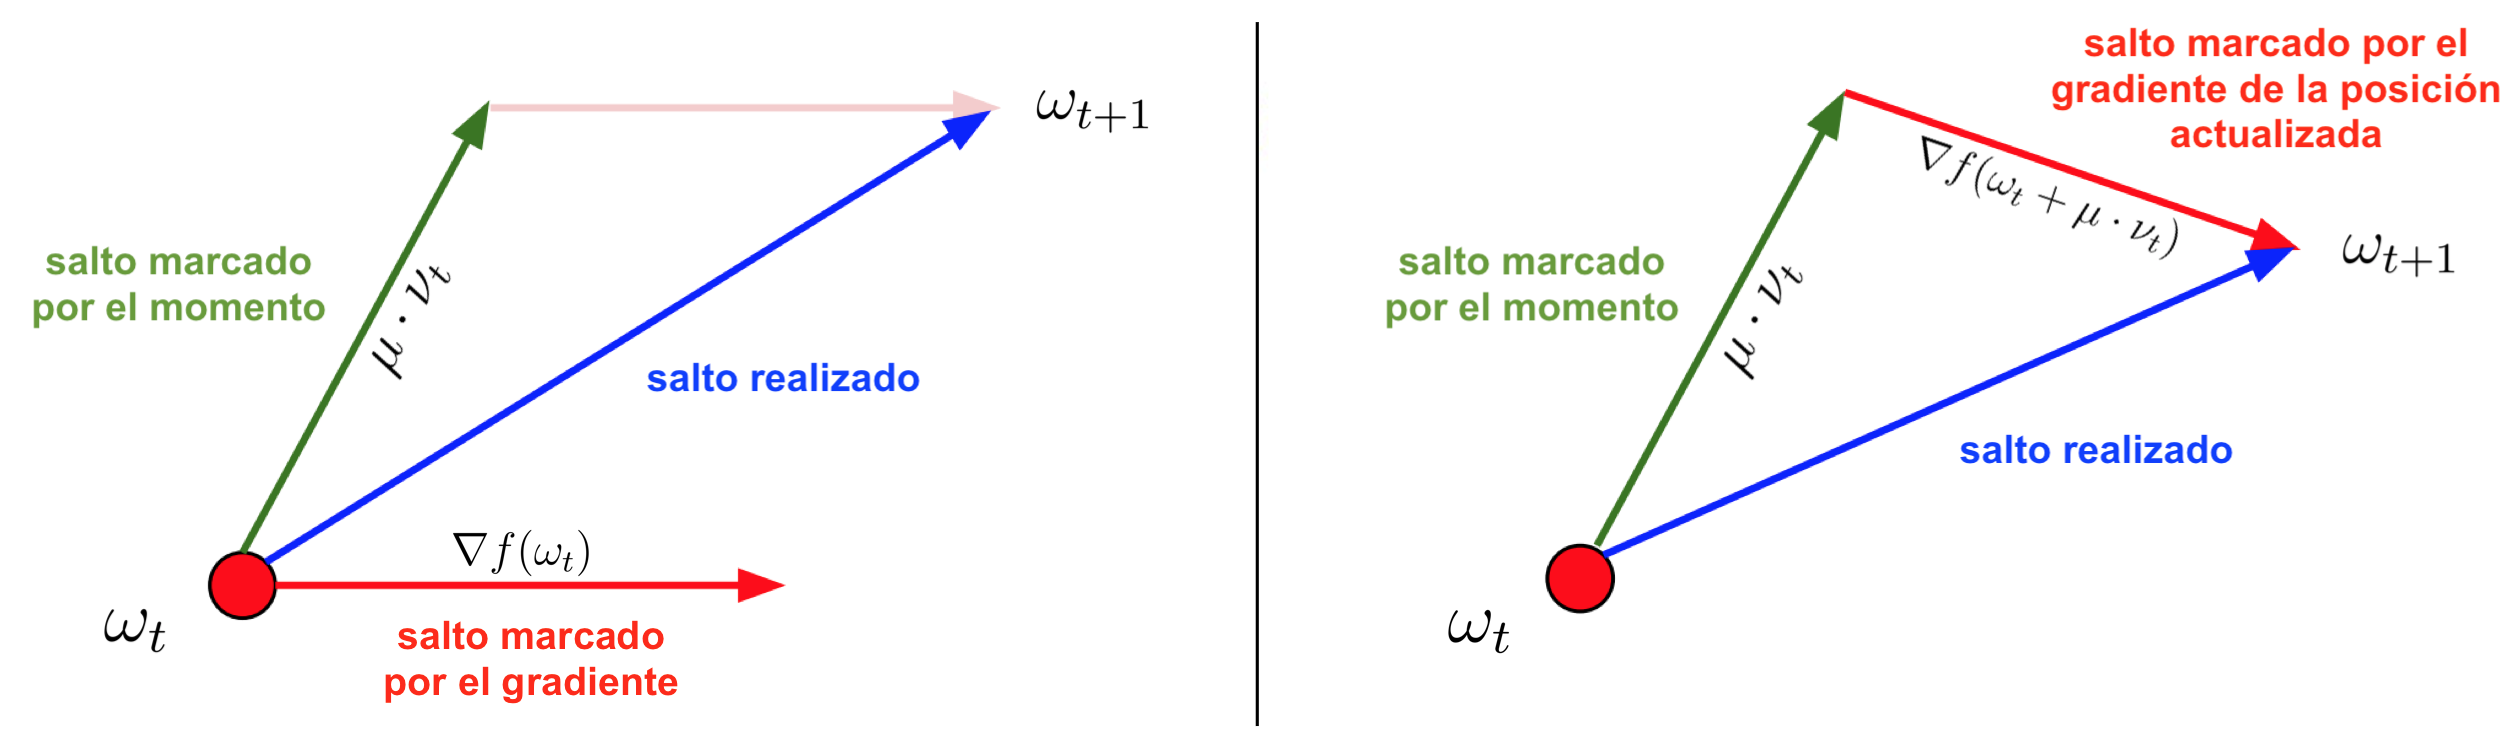
\includegraphics[width=\textwidth]{Images/NesterovMomentum.png}
    \caption{Actualización Momentum (izquierda) y actualización Nesterov Momentum (derecha) \cite{CS231n}.}
    \label{fig:NesterovMomentum}
\end{figure}

Nesterov Momentum, a su vez, también goza de mayores garantías teóricas de convergencia, funcionando ligeramente mejor en la práctica que el método Momentum estándar \cite{Sutskever}. En la \autoref{fig:NesterovMomentum} se puede observar la comparación, haciéndose evidente el aumento de la eficacia de este último procedimiento representado mediante la \autoref{eq:SGDNesterovMomentum}, que da primero los saltos en la dirección del gradiente acumulado anterior para posteriormente calcular el gradiente en la posición actualizada y realizar una corrección.
\begin{align} 
    v_t &= \mu \cdot v_{t-1} - \lambda \cdot \nabla f(\overbrace{\omega_{t-1} + \mu \cdot v_{t-1}}^{w_{salto}}) \label{eq:SGDNM_1} \\
    \overbrace{\omega_t}^{w_{corregido}} &= \omega_{t-1} + v_t \label{eq:SGDNesterovMomentum}
\end{align}

\subsubsection{Estimación del Momento Adaptativo} \label{Chapter:Adam}

Al contrario que el método del descenso estocástico del gradiente, que permite manipular la tasa de aprendizaje de forma global e idéntica para toda la red, Adam adapta la tasa de aprendizaje a cada uno de los parámetros presentes en el modelo. En el artículo que describe este algoritmo, los autores exponen a Adam como la combinación de dos de las extensiones de SGD \cite{Adam}:
\begin{itemize}
  \item Algoritmo de \textbf{Gradiente Adaptativo (AdaGrad)}, el cual presenta una tasa de aprendizaje adaptativa por parámetro que mejora el rendimiento de sistemas con gradientes dispersos, como es el caso de los problemas de visión por computador. 
  \item \textbf{Propagación del Valor Cuadrático Medio (RMSProp)}, que también explota las tasas de aprendizaje adaptativas, basadas en este caso en el promedio de las magnitudes recientes de los gradientes, lo que proporciona buenos resultados para problemas ruidosos. 
\end{itemize}

De esta forma, Adam, además de almacenar un promedio del primer momento (la media), como en RMSProp, también utiliza el promedio de los segundos momentos de los gradientes (la varianza) para la actualización de los parámetros, proceso que se rige por la \autoref{eq:Adam}.
\begin{align}
    m_t &= \beta_1 \cdot m_{t-1} + (1 - \beta_1) \cdot \nabla f(\omega_{t-1}) \label{eq:AdamBeta1}\\
    v_t &= \beta_2 \cdot v_{t-1} + (1 - \beta_2) \cdot \nabla^2 f(\omega_{t-1}) \label{eq:AdamBeta2}\\
    \hat{m}_t &= m_t / (1 - \beta_1^t) \\
    \hat{v}_t &= v_t / (1 - \beta_2^t) \\
    \omega_t &= \omega_{t-1} - \lambda \cdot \hat{m}_t / (\sqrt{\hat{v}_t} + \epsilon) \label{eq:Adam} \\
    \text{donde}~
    \lambda &> 0 \text{\space es la tasa de aprendizaje,} \notag \\
    m_t \text{\space y \space} v_t &\equiv \text{estimaciones del primer y segundo momento,} \notag \\
    \hat{m}_t \text{\space y \space} \hat{v}_t &\equiv \text{estimaciones del primer y segundo momento corregidas} \notag
\end{align}
De forma específica, este algoritmo englobado en la \autoref{eq:Adam} calcula en un primer momento un promedio exponencial del gradiente ($m_t$) y del gradiente cuadrado ($v_t$), cuyas tasas de descenso son controladas mediante los parámetros $\beta_1$ y $\beta_2$. Por otro lado, como $m_t$ y $v_t$ son inicialmente nulos, es necesario aplicarles una corrección para evitar su sesgado hacia cero, especialmente notable durante las primeras iteraciones. Tras ello, se realiza la actualización de los parámetros de manera análoga al método del descenso estocástico del gradiente.

\section{Trabajos Relacionados} \label{Chapter:RelatedWork}

La tarea del reconocimiento de expresiones faciales puede abordarse desde múltiples puntos de vista, abarcando áreas como el procesamiento de señales, la visión por computador o el aprendizaje automático. Precisamente la combinación de estas técnicas es la que ofrece el entorno idóneo para el desarrollo e implementación de los sistemas de identificación de emociones.

En estas circunstancias, es destacable la labor del grupo de investigación comercial Affectiva, que es el líder mundial en reconocimiento de emociones. Su metodología se basa en técnicas de aprendizaje profundo aplicadas a la detección y seguimiento de rostros, a la transcripción de conversaciones, a la detección de la voz y a la clasificación de las emociones a partir de las expresiones faciales y del habla. Además, cabe destacar que los servicios ofrecidos por esta compañía son independientes de factores culturales o regionales dada la extensión de sus bases de datos \cite{Affectiva}, contando, por ejemplo, con casi 6 millones de representaciones faciales de 75 países diferentes. Este número es extraordinariamente elevado teniendo en cuenta que la mayoría de los conjuntos de entrenamiento públicos ni si quiera alcanzan las 5\,0000 imágenes.

En lo que respecta a un enfoque más similar a lo desarrollado en este escrito, tanto por el uso de la misma base de datos (FER-2013 \cite{FER-2013}, analizada en profundidad en la \autoref{Chapter:FER-2013}) como por la metodología empleada, es necesario señalar las siguientes implementaciones:
\begin{itemize}
  \item \textbf{Reconocimiento de Expresión Faciales utilizando Redes Neuronales Convolucionales: Estado del Arte \cite{Pramerdorfer}}. Este modelo, que actualmente está reconocido como el estado del arte en el ámbito del desafío FER-2013, es el resultado de la superación de una serie de cuellos de botella de los sistemas convolucionales (irregularidad de los datos, profundidad de la red, etc.). Su arquitectura está formada por un conjunto de CNNs ensambladas y basadas en modelos actuales y profundos (VGG, Inception y ResNet), así como por una serie de módulos de preprocesamiento que extraen distintos puntos de referencia de interés, igualan el histograma o realizan ajustes lineales a los datos de entrada. La precisión alcanzada por este sistema sobre el conjunto de evaluación de la base de datos FER-2013, sin otros entrenamientos auxiliares anteriores, ha sido de 75.20\%.
  \item \textbf{Aprendiendo los Rasgos de las Relaciones Sociales a partir de Imágenes Faciales \cite{Zhang}}. El modelo aquí descrito desarrolla una serie de técnicas de clasificación y extracción de características basadas en una CNN convencional y una capa adicional y paralela al modelo cuya influencia recae únicamente en la capa de decisión. Mediante esta implementación tan peculiar se pretende fusionar los datos de múltiples fuentes y conseguir, de esta forma, una aproximación espacial de las representaciones de los rostros aprendidos de clases afines. El rendimiento obtenido fue de 75.10\%.
  \item \textbf{Aprendizaje Profundo utilizando Máquinas de Vector de Soporte \cite{DeepSVM}}. El sistema presentado en este documento fue precisamente el ganador del desafío de reconocimiento de expresiones faciales (FER-2013) con una tasa de acierto de 71.16\%. Se caracteriza principalmente por combinar las redes neuronales y las SVM, minimizando, por lo tanto, una función de pérdidas basada en los márgenes de decisión en lugar de la entropía cruzada.
  \item \textbf{Clasificación de Emociones con Aumento de Datos mediante Redes Generativas Antagónicas \cite{GANAugmentation}}. La técnica propuesta en este artículo surge como resultado del estancamiento de los avances en el reconocimiento de expresiones faciales debido a las limitaciones de las bases de datos públicas existentes. Por ello, para complementar el conjunto de entrenamiento se ha propuesto una Red Generativa Antagónica de Ciclo Consecuente (CycleGAN) \cite{cycleGAN} con la que se consigue aumentar la variedad de datos, así como los márgenes entre clases semejantes. Los resultados empíricos han mostrado que es posible obtener un aumento de entre el 5\% y el 10\% en la tasa de acierto empleando estas técnicas.
  \item \textbf{Redes Neuronales Convolucionales para la Clasificación de Emociones y Género en Tiempo Real \cite{Arriaga}}. En este documento se expone un marco de implementación consistente en una red neuronal convolucional que realiza las tareas de detección de rostros, clasificación de género y predicción de emociones en tiempo real. La red propuesta está inspirada en la arquitectura Xception \cite{Xception}, que combina módulos convolucionales separables en profundidad y módulos residuales. La precisión obtenida sobre el conjunto de evaluación de expresiones faciales FER-2013 ha sido de 66\%.
\end{itemize}

Como puede observarse, dada la estandarización de la evaluación de todos estos modelos debido a las características de la base de datos empleada, dividida en tres subconjuntos (entrenamiento, validación y evaluación), los resultados que se van a presentar a lo largo de este proyecto van a poder compararse de forma directa con las tasas anteriormente mencionadas.